% Created by tikzDevice version 0.12.6 on 2025-04-02 10:50:21
% !TEX encoding = UTF-8 Unicode
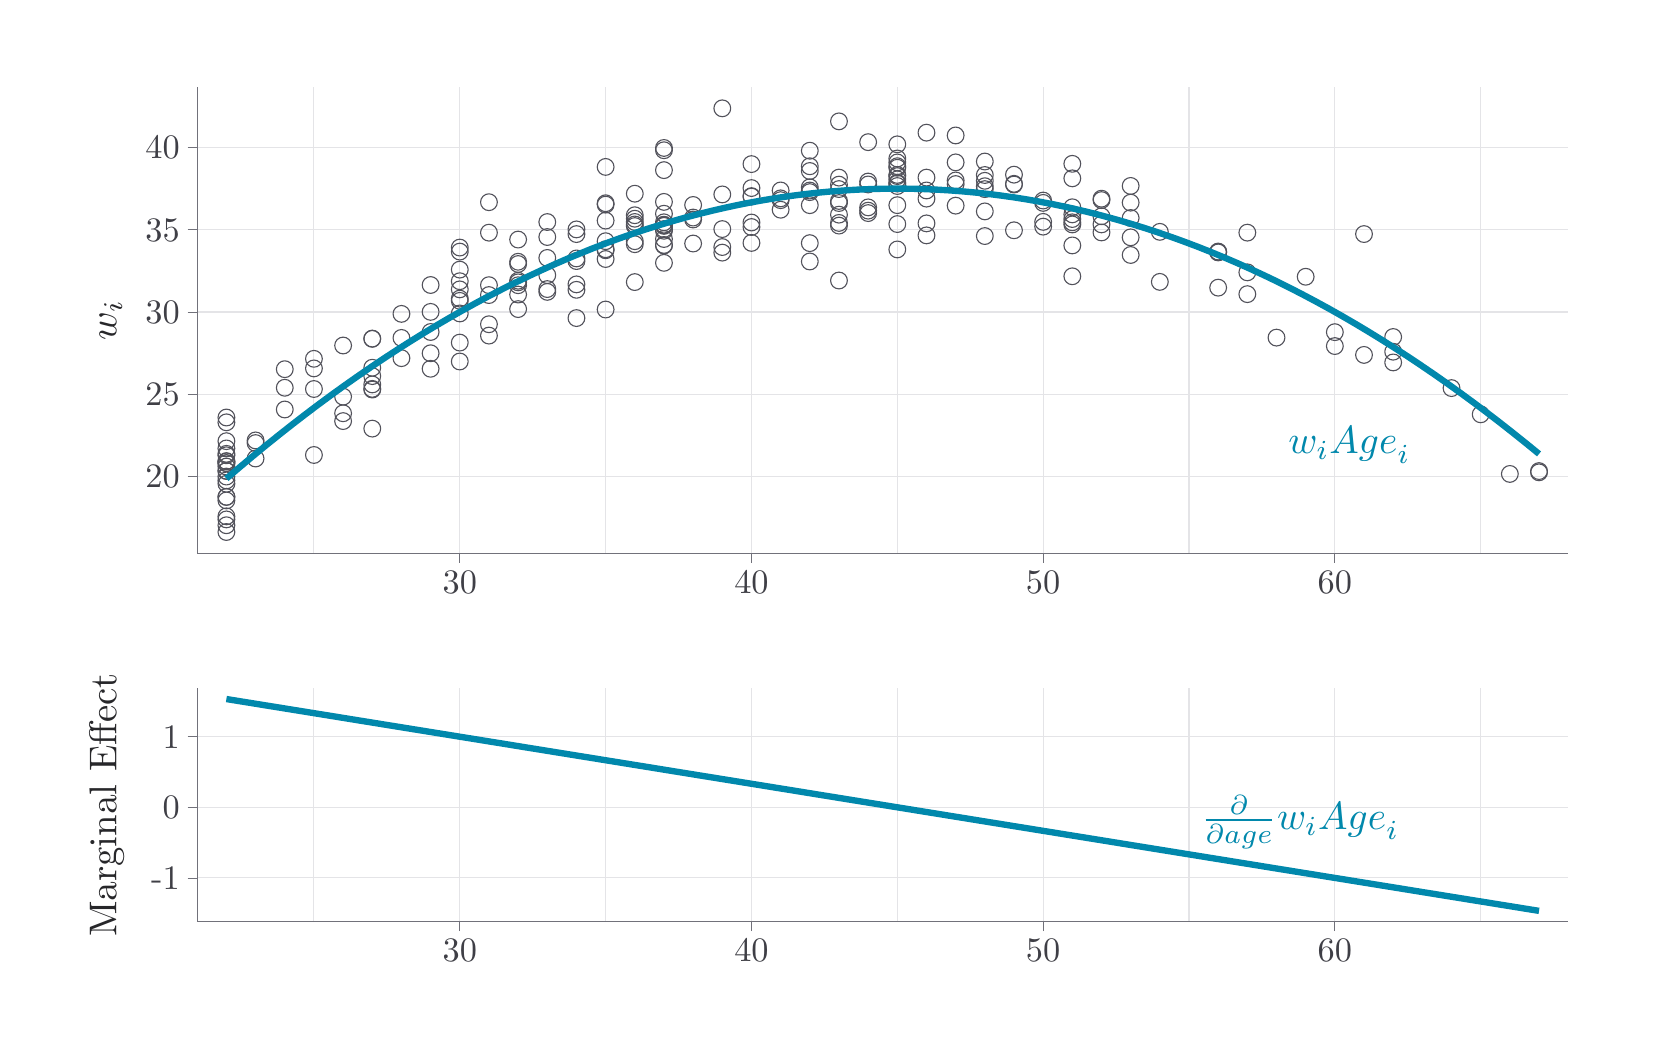
\begin{tikzpicture}[x=1pt,y=1pt]
\definecolor{fillColor}{RGB}{255,255,255}
\path[use as bounding box,fill=fillColor] (0,0) rectangle (578.16,361.35);
\begin{scope}
\path[clip] (  0.00,  0.00) rectangle (578.16,361.35);
\definecolor{drawColor}{RGB}{255,255,255}

\path[draw=drawColor,line width= 0.6pt,line join=round,line cap=round,fill=fillColor] (  0.00,  0.00) rectangle (578.16,361.35);
\end{scope}
\begin{scope}
\path[clip] (  5.50,138.58) rectangle (572.66,355.85);
\definecolor{drawColor}{RGB}{255,255,255}
\definecolor{fillColor}{RGB}{255,255,255}

\path[draw=drawColor,line width= 0.7pt,line join=round,line cap=round,fill=fillColor] (  5.50,138.58) rectangle (572.66,355.85);
\end{scope}
\begin{scope}
\path[clip] (  5.50,  5.50) rectangle (572.66,138.58);
\definecolor{drawColor}{RGB}{255,255,255}
\definecolor{fillColor}{RGB}{255,255,255}

\path[draw=drawColor,line width= 0.7pt,line join=round,line cap=round,fill=fillColor] (  5.50,  5.50) rectangle (572.66,138.58);
\end{scope}
\begin{scope}
\path[clip] ( 61.27,171.46) rectangle (556.66,339.85);
\definecolor{drawColor}{RGB}{255,255,255}
\definecolor{fillColor}{RGB}{255,255,255}

\path[draw=drawColor,line width= 0.7pt,line join=round,line cap=round,fill=fillColor] ( 61.27,171.46) rectangle (556.66,339.85);
\definecolor{drawColor}{RGB}{228,228,231}

\path[draw=drawColor,line width= 0.4pt,line join=round] (103.44,171.46) --
	(103.44,339.85);

\path[draw=drawColor,line width= 0.4pt,line join=round] (208.84,171.46) --
	(208.84,339.85);

\path[draw=drawColor,line width= 0.4pt,line join=round] (314.24,171.46) --
	(314.24,339.85);

\path[draw=drawColor,line width= 0.4pt,line join=round] (419.64,171.46) --
	(419.64,339.85);

\path[draw=drawColor,line width= 0.4pt,line join=round] (525.04,171.46) --
	(525.04,339.85);

\path[draw=drawColor,line width= 0.4pt,line join=round] ( 61.27,199.20) --
	(556.66,199.20);

\path[draw=drawColor,line width= 0.4pt,line join=round] ( 61.27,228.91) --
	(556.66,228.91);

\path[draw=drawColor,line width= 0.4pt,line join=round] ( 61.27,258.62) --
	(556.66,258.62);

\path[draw=drawColor,line width= 0.4pt,line join=round] ( 61.27,288.33) --
	(556.66,288.33);

\path[draw=drawColor,line width= 0.4pt,line join=round] ( 61.27,318.04) --
	(556.66,318.04);

\path[draw=drawColor,line width= 0.4pt,line join=round] (156.14,171.46) --
	(156.14,339.85);

\path[draw=drawColor,line width= 0.4pt,line join=round] (261.54,171.46) --
	(261.54,339.85);

\path[draw=drawColor,line width= 0.4pt,line join=round] (366.94,171.46) --
	(366.94,339.85);

\path[draw=drawColor,line width= 0.4pt,line join=round] (472.34,171.46) --
	(472.34,339.85);
\definecolor{drawColor}{RGB}{82,82,91}

\path[draw=drawColor,line width= 0.4pt,line join=round,line cap=round] (187.76,265.88) circle (  3.03);

\path[draw=drawColor,line width= 0.4pt,line join=round,line cap=round] (103.44,241.69) circle (  3.03);

\path[draw=drawColor,line width= 0.4pt,line join=round,line cap=round] (229.92,282.83) circle (  3.03);

\path[draw=drawColor,line width= 0.4pt,line join=round,line cap=round] (229.92,298.39) circle (  3.03);

\path[draw=drawColor,line width= 0.4pt,line join=round,line cap=round] (187.76,271.93) circle (  3.03);

\path[draw=drawColor,line width= 0.4pt,line join=round,line cap=round] (314.24,310.73) circle (  3.03);

\path[draw=drawColor,line width= 0.4pt,line join=round,line cap=round] (293.16,297.98) circle (  3.03);

\path[draw=drawColor,line width= 0.4pt,line join=round,line cap=round] (166.68,268.30) circle (  3.03);

\path[draw=drawColor,line width= 0.4pt,line join=round,line cap=round] ( 71.81,191.81) circle (  3.03);

\path[draw=drawColor,line width= 0.4pt,line join=round,line cap=round] (335.32,304.84) circle (  3.03);

\path[draw=drawColor,line width= 0.4pt,line join=round,line cap=round] (156.14,263.44) circle (  3.03);

\path[draw=drawColor,line width= 0.4pt,line join=round,line cap=round] (293.16,290.79) circle (  3.03);

\path[draw=drawColor,line width= 0.4pt,line join=round,line cap=round] (335.32,322.40) circle (  3.03);

\path[draw=drawColor,line width= 0.4pt,line join=round,line cap=round] (493.42,240.38) circle (  3.03);

\path[draw=drawColor,line width= 0.4pt,line join=round,line cap=round] ( 71.81,211.93) circle (  3.03);

\path[draw=drawColor,line width= 0.4pt,line join=round,line cap=round] (156.14,240.72) circle (  3.03);

\path[draw=drawColor,line width= 0.4pt,line join=round,line cap=round] (430.18,267.40) circle (  3.03);

\path[draw=drawColor,line width= 0.4pt,line join=round,line cap=round] (398.56,304.16) circle (  3.03);

\path[draw=drawColor,line width= 0.4pt,line join=round,line cap=round] (208.84,281.28) circle (  3.03);

\path[draw=drawColor,line width= 0.4pt,line join=round,line cap=round] (113.98,246.50) circle (  3.03);

\path[draw=drawColor,line width= 0.4pt,line join=round,line cap=round] (187.76,278.14) circle (  3.03);

\path[draw=drawColor,line width= 0.4pt,line join=round,line cap=round] ( 71.81,190.51) circle (  3.03);

\path[draw=drawColor,line width= 0.4pt,line join=round,line cap=round] (156.14,280.43) circle (  3.03);

\path[draw=drawColor,line width= 0.4pt,line join=round,line cap=round] (388.02,293.20) circle (  3.03);

\path[draw=drawColor,line width= 0.4pt,line join=round,line cap=round] (282.62,301.92) circle (  3.03);

\path[draw=drawColor,line width= 0.4pt,line join=round,line cap=round] (335.32,312.67) circle (  3.03);

\path[draw=drawColor,line width= 0.4pt,line join=round,line cap=round] (377.48,271.51) circle (  3.03);

\path[draw=drawColor,line width= 0.4pt,line join=round,line cap=round] (229.92,288.56) circle (  3.03);

\path[draw=drawColor,line width= 0.4pt,line join=round,line cap=round] ( 71.81,209.30) circle (  3.03);

\path[draw=drawColor,line width= 0.4pt,line join=round,line cap=round] (240.46,283.35) circle (  3.03);

\path[draw=drawColor,line width= 0.4pt,line join=round,line cap=round] (314.24,306.54) circle (  3.03);

\path[draw=drawColor,line width= 0.4pt,line join=round,line cap=round] ( 92.90,237.94) circle (  3.03);

\path[draw=drawColor,line width= 0.4pt,line join=round,line cap=round] (366.94,289.45) circle (  3.03);

\path[draw=drawColor,line width= 0.4pt,line join=round,line cap=round] (229.92,289.96) circle (  3.03);

\path[draw=drawColor,line width= 0.4pt,line join=round,line cap=round] (293.16,293.78) circle (  3.03);

\path[draw=drawColor,line width= 0.4pt,line join=round,line cap=round] (398.56,298.12) circle (  3.03);

\path[draw=drawColor,line width= 0.4pt,line join=round,line cap=round] (546.12,201.12) circle (  3.03);

\path[draw=drawColor,line width= 0.4pt,line join=round,line cap=round] (208.84,280.92) circle (  3.03);

\path[draw=drawColor,line width= 0.4pt,line join=round,line cap=round] (219.38,289.66) circle (  3.03);

\path[draw=drawColor,line width= 0.4pt,line join=round,line cap=round] (377.48,296.45) circle (  3.03);

\path[draw=drawColor,line width= 0.4pt,line join=round,line cap=round] (219.38,301.35) circle (  3.03);

\path[draw=drawColor,line width= 0.4pt,line join=round,line cap=round] (229.92,276.37) circle (  3.03);

\path[draw=drawColor,line width= 0.4pt,line join=round,line cap=round] (113.98,228.01) circle (  3.03);

\path[draw=drawColor,line width= 0.4pt,line join=round,line cap=round] (229.92,289.72) circle (  3.03);

\path[draw=drawColor,line width= 0.4pt,line join=round,line cap=round] (314.24,312.65) circle (  3.03);

\path[draw=drawColor,line width= 0.4pt,line join=round,line cap=round] (113.98,219.19) circle (  3.03);

\path[draw=drawColor,line width= 0.4pt,line join=round,line cap=round] (430.18,280.25) circle (  3.03);

\path[draw=drawColor,line width= 0.4pt,line join=round,line cap=round] (166.68,264.73) circle (  3.03);

\path[draw=drawColor,line width= 0.4pt,line join=round,line cap=round] ( 71.81,201.16) circle (  3.03);

\path[draw=drawColor,line width= 0.4pt,line join=round,line cap=round] (240.46,297.28) circle (  3.03);

\path[draw=drawColor,line width= 0.4pt,line join=round,line cap=round] (219.38,290.23) circle (  3.03);

\path[draw=drawColor,line width= 0.4pt,line join=round,line cap=round] (198.30,268.59) circle (  3.03);

\path[draw=drawColor,line width= 0.4pt,line join=round,line cap=round] (482.88,243.10) circle (  3.03);

\path[draw=drawColor,line width= 0.4pt,line join=round,line cap=round] (388.02,290.26) circle (  3.03);

\path[draw=drawColor,line width= 0.4pt,line join=round,line cap=round] (282.62,316.89) circle (  3.03);

\path[draw=drawColor,line width= 0.4pt,line join=round,line cap=round] ( 82.35,212.20) circle (  3.03);

\path[draw=drawColor,line width= 0.4pt,line join=round,line cap=round] ( 71.81,181.55) circle (  3.03);

\path[draw=drawColor,line width= 0.4pt,line join=round,line cap=round] (388.02,299.04) circle (  3.03);

\path[draw=drawColor,line width= 0.4pt,line join=round,line cap=round] (219.38,291.14) circle (  3.03);

\path[draw=drawColor,line width= 0.4pt,line join=round,line cap=round] (314.24,319.19) circle (  3.03);

\path[draw=drawColor,line width= 0.4pt,line join=round,line cap=round] ( 71.81,220.48) circle (  3.03);

\path[draw=drawColor,line width= 0.4pt,line join=round,line cap=round] (535.58,200.09) circle (  3.03);

\path[draw=drawColor,line width= 0.4pt,line join=round,line cap=round] (303.70,294.35) circle (  3.03);

\path[draw=drawColor,line width= 0.4pt,line join=round,line cap=round] (314.24,305.01) circle (  3.03);

\path[draw=drawColor,line width= 0.4pt,line join=round,line cap=round] (156.14,269.73) circle (  3.03);

\path[draw=drawColor,line width= 0.4pt,line join=round,line cap=round] (261.54,303.39) circle (  3.03);

\path[draw=drawColor,line width= 0.4pt,line join=round,line cap=round] (282.62,276.86) circle (  3.03);

\path[draw=drawColor,line width= 0.4pt,line join=round,line cap=round] (198.30,256.41) circle (  3.03);

\path[draw=drawColor,line width= 0.4pt,line join=round,line cap=round] (156.14,247.55) circle (  3.03);

\path[draw=drawColor,line width= 0.4pt,line join=round,line cap=round] (229.92,287.96) circle (  3.03);

\path[draw=drawColor,line width= 0.4pt,line join=round,line cap=round] (345.86,308.11) circle (  3.03);

\path[draw=drawColor,line width= 0.4pt,line join=round,line cap=round] (440.72,272.93) circle (  3.03);

\path[draw=drawColor,line width= 0.4pt,line join=round,line cap=round] ( 71.81,202.76) circle (  3.03);

\path[draw=drawColor,line width= 0.4pt,line join=round,line cap=round] (356.40,308.23) circle (  3.03);

\path[draw=drawColor,line width= 0.4pt,line join=round,line cap=round] ( 71.81,179.11) circle (  3.03);

\path[draw=drawColor,line width= 0.4pt,line join=round,line cap=round] (229.92,290.15) circle (  3.03);

\path[draw=drawColor,line width= 0.4pt,line join=round,line cap=round] (187.76,266.89) circle (  3.03);

\path[draw=drawColor,line width= 0.4pt,line join=round,line cap=round] (356.40,304.66) circle (  3.03);

\path[draw=drawColor,line width= 0.4pt,line join=round,line cap=round] (156.14,266.78) circle (  3.03);

\path[draw=drawColor,line width= 0.4pt,line join=round,line cap=round] ( 82.35,205.67) circle (  3.03);

\path[draw=drawColor,line width= 0.4pt,line join=round,line cap=round] (124.52,238.46) circle (  3.03);

\path[draw=drawColor,line width= 0.4pt,line join=round,line cap=round] (261.54,300.48) circle (  3.03);

\path[draw=drawColor,line width= 0.4pt,line join=round,line cap=round] (124.52,230.58) circle (  3.03);

\path[draw=drawColor,line width= 0.4pt,line join=round,line cap=round] (314.24,281.21) circle (  3.03);

\path[draw=drawColor,line width= 0.4pt,line join=round,line cap=round] (388.02,287.35) circle (  3.03);

\path[draw=drawColor,line width= 0.4pt,line join=round,line cap=round] (124.52,248.91) circle (  3.03);

\path[draw=drawColor,line width= 0.4pt,line join=round,line cap=round] (345.86,303.01) circle (  3.03);

\path[draw=drawColor,line width= 0.4pt,line join=round,line cap=round] (293.16,307.17) circle (  3.03);

\path[draw=drawColor,line width= 0.4pt,line join=round,line cap=round] (303.70,296.41) circle (  3.03);

\path[draw=drawColor,line width= 0.4pt,line join=round,line cap=round] (366.94,298.88) circle (  3.03);

\path[draw=drawColor,line width= 0.4pt,line join=round,line cap=round] (198.30,288.45) circle (  3.03);

\path[draw=drawColor,line width= 0.4pt,line join=round,line cap=round] (314.24,304.13) circle (  3.03);

\path[draw=drawColor,line width= 0.4pt,line join=round,line cap=round] (451.26,249.35) circle (  3.03);

\path[draw=drawColor,line width= 0.4pt,line join=round,line cap=round] (482.88,286.77) circle (  3.03);

\path[draw=drawColor,line width= 0.4pt,line join=round,line cap=round] (398.56,285.58) circle (  3.03);

\path[draw=drawColor,line width= 0.4pt,line join=round,line cap=round] (177.22,259.66) circle (  3.03);

\path[draw=drawColor,line width= 0.4pt,line join=round,line cap=round] (345.86,312.98) circle (  3.03);

\path[draw=drawColor,line width= 0.4pt,line join=round,line cap=round] (314.24,311.29) circle (  3.03);

\path[draw=drawColor,line width= 0.4pt,line join=round,line cap=round] ( 71.81,204.71) circle (  3.03);

\path[draw=drawColor,line width= 0.4pt,line join=round,line cap=round] ( 71.81,197.74) circle (  3.03);

\path[draw=drawColor,line width= 0.4pt,line join=round,line cap=round] (398.56,292.57) circle (  3.03);

\path[draw=drawColor,line width= 0.4pt,line join=round,line cap=round] (219.38,293.57) circle (  3.03);

\path[draw=drawColor,line width= 0.4pt,line join=round,line cap=round] (219.38,292.31) circle (  3.03);

\path[draw=drawColor,line width= 0.4pt,line join=round,line cap=round] (219.38,269.42) circle (  3.03);

\path[draw=drawColor,line width= 0.4pt,line join=round,line cap=round] ( 71.81,204.00) circle (  3.03);

\path[draw=drawColor,line width= 0.4pt,line join=round,line cap=round] (377.48,306.90) circle (  3.03);

\path[draw=drawColor,line width= 0.4pt,line join=round,line cap=round] (261.54,312.05) circle (  3.03);

\path[draw=drawColor,line width= 0.4pt,line join=round,line cap=round] (314.24,297.21) circle (  3.03);

\path[draw=drawColor,line width= 0.4pt,line join=round,line cap=round] (261.54,300.31) circle (  3.03);

\path[draw=drawColor,line width= 0.4pt,line join=round,line cap=round] ( 92.90,223.38) circle (  3.03);

\path[draw=drawColor,line width= 0.4pt,line join=round,line cap=round] (324.78,302.52) circle (  3.03);

\path[draw=drawColor,line width= 0.4pt,line join=round,line cap=round] (113.98,222.01) circle (  3.03);

\path[draw=drawColor,line width= 0.4pt,line join=round,line cap=round] (229.92,291.02) circle (  3.03);

\path[draw=drawColor,line width= 0.4pt,line join=round,line cap=round] (345.86,294.96) circle (  3.03);

\path[draw=drawColor,line width= 0.4pt,line join=round,line cap=round] (345.86,286.05) circle (  3.03);

\path[draw=drawColor,line width= 0.4pt,line join=round,line cap=round] (335.32,297.03) circle (  3.03);

\path[draw=drawColor,line width= 0.4pt,line join=round,line cap=round] (156.14,258.08) circle (  3.03);

\path[draw=drawColor,line width= 0.4pt,line join=round,line cap=round] (166.68,287.27) circle (  3.03);

\path[draw=drawColor,line width= 0.4pt,line join=round,line cap=round] (177.22,268.28) circle (  3.03);

\path[draw=drawColor,line width= 0.4pt,line join=round,line cap=round] (198.30,266.62) circle (  3.03);

\path[draw=drawColor,line width= 0.4pt,line join=round,line cap=round] (145.60,238.09) circle (  3.03);

\path[draw=drawColor,line width= 0.4pt,line join=round,line cap=round] (272.08,302.52) circle (  3.03);

\path[draw=drawColor,line width= 0.4pt,line join=round,line cap=round] (208.84,284.19) circle (  3.03);

\path[draw=drawColor,line width= 0.4pt,line join=round,line cap=round] (356.40,304.92) circle (  3.03);

\path[draw=drawColor,line width= 0.4pt,line join=round,line cap=round] (251.00,280.06) circle (  3.03);

\path[draw=drawColor,line width= 0.4pt,line join=round,line cap=round] (377.48,290.24) circle (  3.03);

\path[draw=drawColor,line width= 0.4pt,line join=round,line cap=round] (208.84,291.63) circle (  3.03);

\path[draw=drawColor,line width= 0.4pt,line join=round,line cap=round] (251.00,301.09) circle (  3.03);

\path[draw=drawColor,line width= 0.4pt,line join=round,line cap=round] (208.84,259.50) circle (  3.03);

\path[draw=drawColor,line width= 0.4pt,line join=round,line cap=round] (303.70,305.74) circle (  3.03);

\path[draw=drawColor,line width= 0.4pt,line join=round,line cap=round] (377.48,291.01) circle (  3.03);

\path[draw=drawColor,line width= 0.4pt,line join=round,line cap=round] (208.84,297.90) circle (  3.03);

\path[draw=drawColor,line width= 0.4pt,line join=round,line cap=round] (124.52,235.44) circle (  3.03);

\path[draw=drawColor,line width= 0.4pt,line join=round,line cap=round] (198.30,286.76) circle (  3.03);

\path[draw=drawColor,line width= 0.4pt,line join=round,line cap=round] (124.52,249.00) circle (  3.03);

\path[draw=drawColor,line width= 0.4pt,line join=round,line cap=round] (251.00,332.20) circle (  3.03);

\path[draw=drawColor,line width= 0.4pt,line join=round,line cap=round] (409.10,269.49) circle (  3.03);

\path[draw=drawColor,line width= 0.4pt,line join=round,line cap=round] (282.62,311.26) circle (  3.03);

\path[draw=drawColor,line width= 0.4pt,line join=round,line cap=round] (461.80,271.34) circle (  3.03);

\path[draw=drawColor,line width= 0.4pt,line join=round,line cap=round] (345.86,306.01) circle (  3.03);

\path[draw=drawColor,line width= 0.4pt,line join=round,line cap=round] (282.62,309.56) circle (  3.03);

\path[draw=drawColor,line width= 0.4pt,line join=round,line cap=round] (251.00,282.08) circle (  3.03);

\path[draw=drawColor,line width= 0.4pt,line join=round,line cap=round] (219.38,284.19) circle (  3.03);

\path[draw=drawColor,line width= 0.4pt,line join=round,line cap=round] (356.40,288.13) circle (  3.03);

\path[draw=drawColor,line width= 0.4pt,line join=round,line cap=round] (198.30,277.96) circle (  3.03);

\path[draw=drawColor,line width= 0.4pt,line join=round,line cap=round] ( 71.81,218.74) circle (  3.03);

\path[draw=drawColor,line width= 0.4pt,line join=round,line cap=round] (493.42,249.57) circle (  3.03);

\path[draw=drawColor,line width= 0.4pt,line join=round,line cap=round] (324.78,290.63) circle (  3.03);

\path[draw=drawColor,line width= 0.4pt,line join=round,line cap=round] (208.84,311.03) circle (  3.03);

\path[draw=drawColor,line width= 0.4pt,line join=round,line cap=round] (293.16,289.83) circle (  3.03);

\path[draw=drawColor,line width= 0.4pt,line join=round,line cap=round] (124.52,230.83) circle (  3.03);

\path[draw=drawColor,line width= 0.4pt,line join=round,line cap=round] (208.84,297.41) circle (  3.03);

\path[draw=drawColor,line width= 0.4pt,line join=round,line cap=round] (240.46,292.73) circle (  3.03);

\path[draw=drawColor,line width= 0.4pt,line join=round,line cap=round] (135.06,249.24) circle (  3.03);

\path[draw=drawColor,line width= 0.4pt,line join=round,line cap=round] ( 71.81,184.77) circle (  3.03);

\path[draw=drawColor,line width= 0.4pt,line join=round,line cap=round] (272.08,299.67) circle (  3.03);

\path[draw=drawColor,line width= 0.4pt,line join=round,line cap=round] (293.16,303.03) circle (  3.03);

\path[draw=drawColor,line width= 0.4pt,line join=round,line cap=round] (261.54,283.57) circle (  3.03);

\path[draw=drawColor,line width= 0.4pt,line join=round,line cap=round] (314.24,314.07) circle (  3.03);

\path[draw=drawColor,line width= 0.4pt,line join=round,line cap=round] (440.72,265.06) circle (  3.03);

\path[draw=drawColor,line width= 0.4pt,line join=round,line cap=round] (124.52,232.43) circle (  3.03);

\path[draw=drawColor,line width= 0.4pt,line join=round,line cap=round] (208.84,277.75) circle (  3.03);

\path[draw=drawColor,line width= 0.4pt,line join=round,line cap=round] (472.34,246.30) circle (  3.03);

\path[draw=drawColor,line width= 0.4pt,line join=round,line cap=round] (229.92,294.11) circle (  3.03);

\path[draw=drawColor,line width= 0.4pt,line join=round,line cap=round] ( 92.90,231.23) circle (  3.03);

\path[draw=drawColor,line width= 0.4pt,line join=round,line cap=round] (303.70,319.98) circle (  3.03);

\path[draw=drawColor,line width= 0.4pt,line join=round,line cap=round] (272.08,299.02) circle (  3.03);

\path[draw=drawColor,line width= 0.4pt,line join=round,line cap=round] (324.78,323.41) circle (  3.03);

\path[draw=drawColor,line width= 0.4pt,line join=round,line cap=round] (388.02,299.55) circle (  3.03);

\path[draw=drawColor,line width= 0.4pt,line join=round,line cap=round] (187.76,285.70) circle (  3.03);

\path[draw=drawColor,line width= 0.4pt,line join=round,line cap=round] (198.30,277.01) circle (  3.03);

\path[draw=drawColor,line width= 0.4pt,line join=round,line cap=round] (135.06,241.93) circle (  3.03);

\path[draw=drawColor,line width= 0.4pt,line join=round,line cap=round] ( 71.81,203.99) circle (  3.03);

\path[draw=drawColor,line width= 0.4pt,line join=round,line cap=round] (177.22,276.76) circle (  3.03);

\path[draw=drawColor,line width= 0.4pt,line join=round,line cap=round] ( 71.81,201.22) circle (  3.03);

\path[draw=drawColor,line width= 0.4pt,line join=round,line cap=round] (282.62,302.50) circle (  3.03);

\path[draw=drawColor,line width= 0.4pt,line join=round,line cap=round] (103.44,238.22) circle (  3.03);

\path[draw=drawColor,line width= 0.4pt,line join=round,line cap=round] (156.14,281.89) circle (  3.03);

\path[draw=drawColor,line width= 0.4pt,line join=round,line cap=round] (240.46,292.03) circle (  3.03);

\path[draw=drawColor,line width= 0.4pt,line join=round,line cap=round] ( 71.81,196.54) circle (  3.03);

\path[draw=drawColor,line width= 0.4pt,line join=round,line cap=round] (177.22,269.31) circle (  3.03);

\path[draw=drawColor,line width= 0.4pt,line join=round,line cap=round] (229.92,309.87) circle (  3.03);

\path[draw=drawColor,line width= 0.4pt,line join=round,line cap=round] (229.92,317.06) circle (  3.03);

\path[draw=drawColor,line width= 0.4pt,line join=round,line cap=round] (345.86,304.06) circle (  3.03);

\path[draw=drawColor,line width= 0.4pt,line join=round,line cap=round] (366.94,291.17) circle (  3.03);

\path[draw=drawColor,line width= 0.4pt,line join=round,line cap=round] (546.12,200.67) circle (  3.03);

\path[draw=drawColor,line width= 0.4pt,line join=round,line cap=round] (177.22,264.91) circle (  3.03);

\path[draw=drawColor,line width= 0.4pt,line join=round,line cap=round] (272.08,295.56) circle (  3.03);

\path[draw=drawColor,line width= 0.4pt,line join=round,line cap=round] (156.14,262.63) circle (  3.03);

\path[draw=drawColor,line width= 0.4pt,line join=round,line cap=round] (282.62,303.66) circle (  3.03);

\path[draw=drawColor,line width= 0.4pt,line join=round,line cap=round] (377.48,312.15) circle (  3.03);

\path[draw=drawColor,line width= 0.4pt,line join=round,line cap=round] (324.78,299.57) circle (  3.03);

\path[draw=drawColor,line width= 0.4pt,line join=round,line cap=round] (177.22,284.78) circle (  3.03);

\path[draw=drawColor,line width= 0.4pt,line join=round,line cap=round] (377.48,292.20) circle (  3.03);

\path[draw=drawColor,line width= 0.4pt,line join=round,line cap=round] (282.62,283.49) circle (  3.03);

\path[draw=drawColor,line width= 0.4pt,line join=round,line cap=round] ( 71.81,199.14) circle (  3.03);

\path[draw=drawColor,line width= 0.4pt,line join=round,line cap=round] (166.68,250.08) circle (  3.03);

\path[draw=drawColor,line width= 0.4pt,line join=round,line cap=round] (377.48,293.88) circle (  3.03);

\path[draw=drawColor,line width= 0.4pt,line join=round,line cap=round] (251.00,288.57) circle (  3.03);

\path[draw=drawColor,line width= 0.4pt,line join=round,line cap=round] (377.48,282.66) circle (  3.03);

\path[draw=drawColor,line width= 0.4pt,line join=round,line cap=round] (324.78,286.29) circle (  3.03);

\path[draw=drawColor,line width= 0.4pt,line join=round,line cap=round] ( 82.35,211.24) circle (  3.03);

\path[draw=drawColor,line width= 0.4pt,line join=round,line cap=round] (409.10,287.57) circle (  3.03);

\path[draw=drawColor,line width= 0.4pt,line join=round,line cap=round] (430.18,280.45) circle (  3.03);

\path[draw=drawColor,line width= 0.4pt,line join=round,line cap=round] (430.18,280.14) circle (  3.03);

\path[draw=drawColor,line width= 0.4pt,line join=round,line cap=round] (229.92,317.88) circle (  3.03);

\path[draw=drawColor,line width= 0.4pt,line join=round,line cap=round] (303.70,295.23) circle (  3.03);

\path[draw=drawColor,line width= 0.4pt,line join=round,line cap=round] (229.92,284.98) circle (  3.03);

\path[draw=drawColor,line width= 0.4pt,line join=round,line cap=round] (156.14,273.92) circle (  3.03);

\path[draw=drawColor,line width= 0.4pt,line join=round,line cap=round] (314.24,290.38) circle (  3.03);

\path[draw=drawColor,line width= 0.4pt,line join=round,line cap=round] (525.04,221.63) circle (  3.03);

\path[draw=drawColor,line width= 0.4pt,line join=round,line cap=round] (293.16,304.63) circle (  3.03);

\path[draw=drawColor,line width= 0.4pt,line join=round,line cap=round] ( 71.81,207.35) circle (  3.03);

\path[draw=drawColor,line width= 0.4pt,line join=round,line cap=round] ( 71.81,204.64) circle (  3.03);

\path[draw=drawColor,line width= 0.4pt,line join=round,line cap=round] (229.92,282.63) circle (  3.03);

\path[draw=drawColor,line width= 0.4pt,line join=round,line cap=round] (293.16,298.73) circle (  3.03);

\path[draw=drawColor,line width= 0.4pt,line join=round,line cap=round] (166.68,254.18) circle (  3.03);

\path[draw=drawColor,line width= 0.4pt,line join=round,line cap=round] (440.72,287.28) circle (  3.03);

\path[draw=drawColor,line width= 0.4pt,line join=round,line cap=round] ( 71.81,206.83) circle (  3.03);

\path[draw=drawColor,line width= 0.4pt,line join=round,line cap=round] (124.52,216.47) circle (  3.03);

\path[draw=drawColor,line width= 0.4pt,line join=round,line cap=round] (103.44,230.78) circle (  3.03);

\path[draw=drawColor,line width= 0.4pt,line join=round,line cap=round] (261.54,289.31) circle (  3.03);

\path[draw=drawColor,line width= 0.4pt,line join=round,line cap=round] (472.34,251.32) circle (  3.03);

\path[draw=drawColor,line width= 0.4pt,line join=round,line cap=round] (177.22,275.95) circle (  3.03);

\path[draw=drawColor,line width= 0.4pt,line join=round,line cap=round] (335.32,306.13) circle (  3.03);

\path[draw=drawColor,line width= 0.4pt,line join=round,line cap=round] (314.24,308.14) circle (  3.03);

\path[draw=drawColor,line width= 0.4pt,line join=round,line cap=round] (303.70,304.69) circle (  3.03);

\path[draw=drawColor,line width= 0.4pt,line join=round,line cap=round] (187.76,291.11) circle (  3.03);

\path[draw=drawColor,line width= 0.4pt,line join=round,line cap=round] (293.16,327.49) circle (  3.03);

\path[draw=drawColor,line width= 0.4pt,line join=round,line cap=round] (261.54,290.94) circle (  3.03);

\path[draw=drawColor,line width= 0.4pt,line join=round,line cap=round] (493.42,244.26) circle (  3.03);

\path[draw=drawColor,line width= 0.4pt,line join=round,line cap=round] (514.50,231.11) circle (  3.03);

\path[draw=drawColor,line width= 0.4pt,line join=round,line cap=round] (293.16,269.98) circle (  3.03);

\path[draw=drawColor,line width= 0.4pt,line join=round,line cap=round] ( 71.81,183.66) circle (  3.03);

\path[draw=drawColor,line width= 0.4pt,line join=round,line cap=round] (219.38,283.10) circle (  3.03);

\path[draw=drawColor,line width= 0.4pt,line join=round,line cap=round] (314.24,305.31) circle (  3.03);

\path[draw=drawColor,line width= 0.4pt,line join=round,line cap=round] (366.94,298.03) circle (  3.03);

\path[draw=drawColor,line width= 0.4pt,line join=round,line cap=round] ( 71.81,191.79) circle (  3.03);

\path[draw=drawColor,line width= 0.4pt,line join=round,line cap=round] (135.06,257.93) circle (  3.03);

\path[draw=drawColor,line width= 0.4pt,line join=round,line cap=round] (166.68,298.28) circle (  3.03);

\path[draw=drawColor,line width= 0.4pt,line join=round,line cap=round] (282.62,297.21) circle (  3.03);

\path[draw=drawColor,line width= 0.4pt,line join=round,line cap=round] (145.60,268.36) circle (  3.03);

\path[draw=drawColor,line width= 0.4pt,line join=round,line cap=round] (103.44,206.94) circle (  3.03);

\path[draw=drawColor,line width= 0.4pt,line join=round,line cap=round] (398.56,279.21) circle (  3.03);

\path[draw=drawColor,line width= 0.4pt,line join=round,line cap=round] (145.60,251.38) circle (  3.03);

\path[draw=drawColor,line width= 0.4pt,line join=round,line cap=round] (314.24,307.71) circle (  3.03);

\path[draw=drawColor,line width= 0.4pt,line join=round,line cap=round] (324.78,307.17) circle (  3.03);

\path[draw=drawColor,line width= 0.4pt,line join=round,line cap=round] (145.60,243.70) circle (  3.03);

\path[draw=drawColor,line width= 0.4pt,line join=round,line cap=round] (177.22,269.90) circle (  3.03);

\path[draw=drawColor,line width= 0.4pt,line join=round,line cap=round] (145.60,258.65) circle (  3.03);
\definecolor{drawColor}{RGB}{1,136,172}

\path[draw=drawColor,line width= 2.3pt,line join=round] ( 71.81,198.41) --
	( 76.56,202.47) --
	( 81.30,206.45) --
	( 86.04,210.35) --
	( 90.79,214.17) --
	( 95.53,217.91) --
	(100.27,221.57) --
	(105.02,225.15) --
	(109.76,228.65) --
	(114.50,232.06) --
	(119.25,235.40) --
	(123.99,238.66) --
	(128.73,241.84) --
	(133.47,244.93) --
	(138.22,247.95) --
	(142.96,250.89) --
	(147.70,253.74) --
	(152.45,256.52) --
	(157.19,259.22) --
	(161.93,261.83) --
	(166.68,264.37) --
	(171.42,266.82) --
	(176.16,269.20) --
	(180.90,271.49) --
	(185.65,273.71) --
	(190.39,275.84) --
	(195.13,277.90) --
	(199.88,279.87) --
	(204.62,281.77) --
	(209.36,283.58) --
	(214.11,285.31) --
	(218.85,286.97) --
	(223.59,288.54) --
	(228.34,290.03) --
	(233.08,291.45) --
	(237.82,292.78) --
	(242.56,294.03) --
	(247.31,295.20) --
	(252.05,296.29) --
	(256.79,297.31) --
	(261.54,298.24) --
	(266.28,299.09) --
	(271.02,299.86) --
	(275.77,300.55) --
	(280.51,301.16) --
	(285.25,301.69) --
	(290.00,302.14) --
	(294.74,302.51) --
	(299.48,302.80) --
	(304.22,303.01) --
	(308.97,303.14) --
	(313.71,303.19) --
	(318.45,303.16) --
	(323.20,303.05) --
	(327.94,302.85) --
	(332.68,302.58) --
	(337.43,302.23) --
	(342.17,301.80) --
	(346.91,301.29) --
	(351.65,300.69) --
	(356.40,300.02) --
	(361.14,299.27) --
	(365.88,298.43) --
	(370.63,297.52) --
	(375.37,296.53) --
	(380.11,295.45) --
	(384.86,294.30) --
	(389.60,293.06) --
	(394.34,291.75) --
	(399.09,290.35) --
	(403.83,288.88) --
	(408.57,287.32) --
	(413.31,285.69) --
	(418.06,283.97) --
	(422.80,282.18) --
	(427.54,280.30) --
	(432.29,278.34) --
	(437.03,276.31) --
	(441.77,274.19) --
	(446.52,271.99) --
	(451.26,269.72) --
	(456.00,267.36) --
	(460.74,264.92) --
	(465.49,262.40) --
	(470.23,259.81) --
	(474.97,257.13) --
	(479.72,254.37) --
	(484.46,251.53) --
	(489.20,248.61) --
	(493.95,245.61) --
	(498.69,242.53) --
	(503.43,239.37) --
	(508.18,236.13) --
	(512.92,232.81) --
	(517.66,229.41) --
	(522.40,225.93) --
	(527.15,222.37) --
	(531.89,218.73) --
	(536.63,215.01) --
	(541.38,211.21) --
	(546.12,207.33);

\path[] (424.27,203.13) --
	(501.39,203.13) --
	(501.29,203.13) --
	(501.70,203.15) --
	(502.10,203.23) --
	(502.49,203.38) --
	(502.85,203.58) --
	(503.17,203.84) --
	(503.44,204.15) --
	(503.67,204.50) --
	(503.83,204.88) --
	(503.93,205.29) --
	(503.96,205.70) --
	(503.96,205.70) --
	(503.96,218.46) --
	(503.96,218.46) --
	(503.93,218.87) --
	(503.83,219.27) --
	(503.67,219.65) --
	(503.44,220.00) --
	(503.17,220.31) --
	(502.85,220.58) --
	(502.49,220.78) --
	(502.10,220.93) --
	(501.70,221.01) --
	(501.39,221.03) --
	(424.27,221.03) --
	(424.58,221.01) --
	(424.17,221.03) --
	(423.76,220.98) --
	(423.36,220.86) --
	(422.99,220.69) --
	(422.65,220.45) --
	(422.35,220.16) --
	(422.10,219.83) --
	(421.91,219.47) --
	(421.78,219.07) --
	(421.71,218.67) --
	(421.70,218.46) --
	(421.70,205.70) --
	(421.71,205.90) --
	(421.71,205.49) --
	(421.78,205.08) --
	(421.91,204.69) --
	(422.10,204.32) --
	(422.35,203.99) --
	(422.65,203.71) --
	(422.99,203.47) --
	(423.36,203.29) --
	(423.76,203.18) --
	(424.17,203.13) --
	cycle;
\end{scope}
\begin{scope}
\path[clip] ( 61.27,171.46) rectangle (556.66,339.85);
\definecolor{drawColor}{RGB}{1,136,172}

\node[text=drawColor,anchor=base east,inner sep=0pt, outer sep=0pt, scale=  1.42] at (499.68,207.41) {$\expec{w_i}{\text{Age}_i}$};
\end{scope}
\begin{scope}
\path[clip] (  0.00,  0.00) rectangle (578.16,361.35);
\definecolor{drawColor}{RGB}{113,113,122}

\path[draw=drawColor,line width= 0.3pt,line join=round] ( 61.27,171.46) --
	( 61.27,339.85);
\end{scope}
\begin{scope}
\path[clip] (  0.00,  0.00) rectangle (578.16,361.35);
\definecolor{drawColor}{RGB}{63,63,70}

\node[text=drawColor,anchor=base east,inner sep=0pt, outer sep=0pt, scale=  1.24] at ( 54.97,195.12) {20};

\node[text=drawColor,anchor=base east,inner sep=0pt, outer sep=0pt, scale=  1.24] at ( 54.97,224.83) {25};

\node[text=drawColor,anchor=base east,inner sep=0pt, outer sep=0pt, scale=  1.24] at ( 54.97,254.54) {30};

\node[text=drawColor,anchor=base east,inner sep=0pt, outer sep=0pt, scale=  1.24] at ( 54.97,284.25) {35};

\node[text=drawColor,anchor=base east,inner sep=0pt, outer sep=0pt, scale=  1.24] at ( 54.97,313.96) {40};
\end{scope}
\begin{scope}
\path[clip] (  0.00,  0.00) rectangle (578.16,361.35);
\definecolor{drawColor}{RGB}{113,113,122}

\path[draw=drawColor,line width= 0.3pt,line join=round] ( 57.77,199.20) --
	( 61.27,199.20);

\path[draw=drawColor,line width= 0.3pt,line join=round] ( 57.77,228.91) --
	( 61.27,228.91);

\path[draw=drawColor,line width= 0.3pt,line join=round] ( 57.77,258.62) --
	( 61.27,258.62);

\path[draw=drawColor,line width= 0.3pt,line join=round] ( 57.77,288.33) --
	( 61.27,288.33);

\path[draw=drawColor,line width= 0.3pt,line join=round] ( 57.77,318.04) --
	( 61.27,318.04);
\end{scope}
\begin{scope}
\path[clip] (  0.00,  0.00) rectangle (578.16,361.35);
\definecolor{drawColor}{RGB}{113,113,122}

\path[draw=drawColor,line width= 0.3pt,line join=round] ( 61.27,171.46) --
	(556.66,171.46);
\end{scope}
\begin{scope}
\path[clip] (  0.00,  0.00) rectangle (578.16,361.35);
\definecolor{drawColor}{RGB}{113,113,122}

\path[draw=drawColor,line width= 0.3pt,line join=round] (156.14,167.96) --
	(156.14,171.46);

\path[draw=drawColor,line width= 0.3pt,line join=round] (261.54,167.96) --
	(261.54,171.46);

\path[draw=drawColor,line width= 0.3pt,line join=round] (366.94,167.96) --
	(366.94,171.46);

\path[draw=drawColor,line width= 0.3pt,line join=round] (472.34,167.96) --
	(472.34,171.46);
\end{scope}
\begin{scope}
\path[clip] (  0.00,  0.00) rectangle (578.16,361.35);
\definecolor{drawColor}{RGB}{63,63,70}

\node[text=drawColor,anchor=base,inner sep=0pt, outer sep=0pt, scale=  1.24] at (156.14,156.99) {30};

\node[text=drawColor,anchor=base,inner sep=0pt, outer sep=0pt, scale=  1.24] at (261.54,156.99) {40};

\node[text=drawColor,anchor=base,inner sep=0pt, outer sep=0pt, scale=  1.24] at (366.94,156.99) {50};

\node[text=drawColor,anchor=base,inner sep=0pt, outer sep=0pt, scale=  1.24] at (472.34,156.99) {60};
\end{scope}
\begin{scope}
\path[clip] (  0.00,  0.00) rectangle (578.16,361.35);
\definecolor{drawColor}{RGB}{39,39,42}

\node[text=drawColor,rotate= 90.00,anchor=base,inner sep=0pt, outer sep=0pt, scale=  1.40] at ( 32.04,255.65) {$w_i$};
\end{scope}
\begin{scope}
\path[clip] ( 61.27, 38.38) rectangle (556.66,122.58);
\definecolor{drawColor}{RGB}{255,255,255}
\definecolor{fillColor}{RGB}{255,255,255}

\path[draw=drawColor,line width= 0.7pt,line join=round,line cap=round,fill=fillColor] ( 61.27, 38.38) rectangle (556.66,122.58);
\definecolor{drawColor}{RGB}{228,228,231}

\path[draw=drawColor,line width= 0.4pt,line join=round] (103.44, 38.38) --
	(103.44,122.58);

\path[draw=drawColor,line width= 0.4pt,line join=round] (208.84, 38.38) --
	(208.84,122.58);

\path[draw=drawColor,line width= 0.4pt,line join=round] (314.24, 38.38) --
	(314.24,122.58);

\path[draw=drawColor,line width= 0.4pt,line join=round] (419.64, 38.38) --
	(419.64,122.58);

\path[draw=drawColor,line width= 0.4pt,line join=round] (525.04, 38.38) --
	(525.04,122.58);

\path[draw=drawColor,line width= 0.4pt,line join=round] ( 61.27, 54.11) --
	(556.66, 54.11);

\path[draw=drawColor,line width= 0.4pt,line join=round] ( 61.27, 79.63) --
	(556.66, 79.63);

\path[draw=drawColor,line width= 0.4pt,line join=round] ( 61.27,105.14) --
	(556.66,105.14);

\path[draw=drawColor,line width= 0.4pt,line join=round] (156.14, 38.38) --
	(156.14,122.58);

\path[draw=drawColor,line width= 0.4pt,line join=round] (261.54, 38.38) --
	(261.54,122.58);

\path[draw=drawColor,line width= 0.4pt,line join=round] (366.94, 38.38) --
	(366.94,122.58);

\path[draw=drawColor,line width= 0.4pt,line join=round] (472.34, 38.38) --
	(472.34,122.58);
\definecolor{drawColor}{RGB}{1,136,172}

\path[draw=drawColor,line width= 2.3pt,line join=round] ( 71.81,118.75) --
	( 76.56,117.98) --
	( 81.30,117.22) --
	( 86.04,116.45) --
	( 90.79,115.69) --
	( 95.53,114.92) --
	(100.27,114.16) --
	(105.02,113.39) --
	(109.76,112.63) --
	(114.50,111.86) --
	(119.25,111.09) --
	(123.99,110.33) --
	(128.73,109.56) --
	(133.47,108.80) --
	(138.22,108.03) --
	(142.96,107.27) --
	(147.70,106.50) --
	(152.45,105.74) --
	(157.19,104.97) --
	(161.93,104.21) --
	(166.68,103.44) --
	(171.42,102.68) --
	(176.16,101.91) --
	(180.90,101.14) --
	(185.65,100.38) --
	(190.39, 99.61) --
	(195.13, 98.85) --
	(199.88, 98.08) --
	(204.62, 97.32) --
	(209.36, 96.55) --
	(214.11, 95.79) --
	(218.85, 95.02) --
	(223.59, 94.26) --
	(228.34, 93.49) --
	(233.08, 92.72) --
	(237.82, 91.96) --
	(242.56, 91.19) --
	(247.31, 90.43) --
	(252.05, 89.66) --
	(256.79, 88.90) --
	(261.54, 88.13) --
	(266.28, 87.37) --
	(271.02, 86.60) --
	(275.77, 85.84) --
	(280.51, 85.07) --
	(285.25, 84.30) --
	(290.00, 83.54) --
	(294.74, 82.77) --
	(299.48, 82.01) --
	(304.22, 81.24) --
	(308.97, 80.48) --
	(313.71, 79.71) --
	(318.45, 78.95) --
	(323.20, 78.18) --
	(327.94, 77.42) --
	(332.68, 76.65) --
	(337.43, 75.89) --
	(342.17, 75.12) --
	(346.91, 74.35) --
	(351.65, 73.59) --
	(356.40, 72.82) --
	(361.14, 72.06) --
	(365.88, 71.29) --
	(370.63, 70.53) --
	(375.37, 69.76) --
	(380.11, 69.00) --
	(384.86, 68.23) --
	(389.60, 67.47) --
	(394.34, 66.70) --
	(399.09, 65.93) --
	(403.83, 65.17) --
	(408.57, 64.40) --
	(413.31, 63.64) --
	(418.06, 62.87) --
	(422.80, 62.11) --
	(427.54, 61.34) --
	(432.29, 60.58) --
	(437.03, 59.81) --
	(441.77, 59.05) --
	(446.52, 58.28) --
	(451.26, 57.51) --
	(456.00, 56.75) --
	(460.74, 55.98) --
	(465.49, 55.22) --
	(470.23, 54.45) --
	(474.97, 53.69) --
	(479.72, 52.92) --
	(484.46, 52.16) --
	(489.20, 51.39) --
	(493.95, 50.63) --
	(498.69, 49.86) --
	(503.43, 49.09) --
	(508.18, 48.33) --
	(512.92, 47.56) --
	(517.66, 46.80) --
	(522.40, 46.03) --
	(527.15, 45.27) --
	(531.89, 44.50) --
	(536.63, 43.74) --
	(541.38, 42.97) --
	(546.12, 42.21);

\path[] (422.21, 67.27) --
	(523.42, 67.27) --
	(523.31, 67.28) --
	(523.73, 67.29) --
	(524.13, 67.38) --
	(524.52, 67.52) --
	(524.88, 67.73) --
	(525.20, 67.99) --
	(525.47, 68.30) --
	(525.69, 68.65) --
	(525.85, 69.03) --
	(525.95, 69.43) --
	(525.99, 69.84) --
	(525.99, 69.84) --
	(525.99, 82.61) --
	(525.99, 82.61) --
	(525.95, 83.02) --
	(525.85, 83.42) --
	(525.69, 83.80) --
	(525.47, 84.15) --
	(525.20, 84.46) --
	(524.88, 84.72) --
	(524.52, 84.93) --
	(524.13, 85.08) --
	(523.73, 85.16) --
	(523.42, 85.18) --
	(422.21, 85.18) --
	(422.52, 85.16) --
	(422.11, 85.17) --
	(421.69, 85.12) --
	(421.30, 85.01) --
	(420.92, 84.83) --
	(420.58, 84.60) --
	(420.28, 84.31) --
	(420.04, 83.98) --
	(419.84, 83.61) --
	(419.71, 83.22) --
	(419.65, 82.81) --
	(419.64, 82.61) --
	(419.64, 69.84) --
	(419.65, 70.05) --
	(419.65, 69.64) --
	(419.71, 69.23) --
	(419.84, 68.84) --
	(420.04, 68.47) --
	(420.28, 68.14) --
	(420.58, 67.85) --
	(420.92, 67.62) --
	(421.30, 67.44) --
	(421.69, 67.33) --
	(422.11, 67.28) --
	cycle;
\end{scope}
\begin{scope}
\path[clip] ( 61.27, 38.38) rectangle (556.66,122.58);
\definecolor{drawColor}{RGB}{1,136,172}

\node[text=drawColor,anchor=base west,inner sep=0pt, outer sep=0pt, scale=  1.42] at (423.92, 71.56) {$\frac{\partial}{\partial \text{age}}\expec{w_i}{\text{Age}_i}$};
\end{scope}
\begin{scope}
\path[clip] (  0.00,  0.00) rectangle (578.16,361.35);
\definecolor{drawColor}{RGB}{113,113,122}

\path[draw=drawColor,line width= 0.3pt,line join=round] ( 61.27, 38.38) --
	( 61.27,122.58);
\end{scope}
\begin{scope}
\path[clip] (  0.00,  0.00) rectangle (578.16,361.35);
\definecolor{drawColor}{RGB}{63,63,70}

\node[text=drawColor,anchor=base east,inner sep=0pt, outer sep=0pt, scale=  1.24] at ( 54.97, 50.03) {-1};

\node[text=drawColor,anchor=base east,inner sep=0pt, outer sep=0pt, scale=  1.24] at ( 54.97, 75.55) {0};

\node[text=drawColor,anchor=base east,inner sep=0pt, outer sep=0pt, scale=  1.24] at ( 54.97,101.06) {1};
\end{scope}
\begin{scope}
\path[clip] (  0.00,  0.00) rectangle (578.16,361.35);
\definecolor{drawColor}{RGB}{113,113,122}

\path[draw=drawColor,line width= 0.3pt,line join=round] ( 57.77, 54.11) --
	( 61.27, 54.11);

\path[draw=drawColor,line width= 0.3pt,line join=round] ( 57.77, 79.63) --
	( 61.27, 79.63);

\path[draw=drawColor,line width= 0.3pt,line join=round] ( 57.77,105.14) --
	( 61.27,105.14);
\end{scope}
\begin{scope}
\path[clip] (  0.00,  0.00) rectangle (578.16,361.35);
\definecolor{drawColor}{RGB}{113,113,122}

\path[draw=drawColor,line width= 0.3pt,line join=round] ( 61.27, 38.38) --
	(556.66, 38.38);
\end{scope}
\begin{scope}
\path[clip] (  0.00,  0.00) rectangle (578.16,361.35);
\definecolor{drawColor}{RGB}{113,113,122}

\path[draw=drawColor,line width= 0.3pt,line join=round] (156.14, 34.88) --
	(156.14, 38.38);

\path[draw=drawColor,line width= 0.3pt,line join=round] (261.54, 34.88) --
	(261.54, 38.38);

\path[draw=drawColor,line width= 0.3pt,line join=round] (366.94, 34.88) --
	(366.94, 38.38);

\path[draw=drawColor,line width= 0.3pt,line join=round] (472.34, 34.88) --
	(472.34, 38.38);
\end{scope}
\begin{scope}
\path[clip] (  0.00,  0.00) rectangle (578.16,361.35);
\definecolor{drawColor}{RGB}{63,63,70}

\node[text=drawColor,anchor=base,inner sep=0pt, outer sep=0pt, scale=  1.24] at (156.14, 23.92) {30};

\node[text=drawColor,anchor=base,inner sep=0pt, outer sep=0pt, scale=  1.24] at (261.54, 23.92) {40};

\node[text=drawColor,anchor=base,inner sep=0pt, outer sep=0pt, scale=  1.24] at (366.94, 23.92) {50};

\node[text=drawColor,anchor=base,inner sep=0pt, outer sep=0pt, scale=  1.24] at (472.34, 23.92) {60};
\end{scope}
\begin{scope}
\path[clip] (  0.00,  0.00) rectangle (578.16,361.35);
\definecolor{drawColor}{RGB}{39,39,42}

\node[text=drawColor,rotate= 90.00,anchor=base,inner sep=0pt, outer sep=0pt, scale=  1.40] at ( 32.04, 80.48) {Marginal Effect};
\end{scope}
\end{tikzpicture}
